\begin{center}
  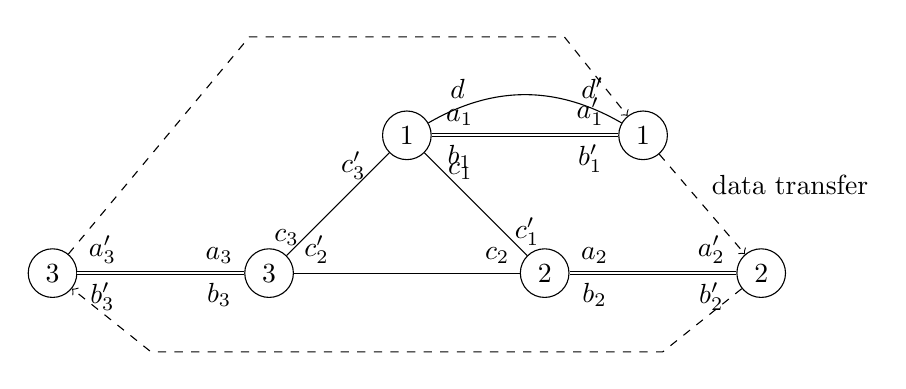
\begin{tikzpicture}
    \node[shape=circle,draw=black] (agent1) at ( 0.00, 0.00) {\tm{\agent1}};
    \node[shape=circle,draw=black] (agent2) at ( 1.75,-1.75) {\tm{\agent2}};
    \node[shape=circle,draw=black] (agent3) at (-1.75,-1.75) {\tm{\agent3}};
    \node[shape=circle,draw=black] (proc1)  at ( 3.00, 0.00) {\tm{\proc1}};
    \node[shape=circle,draw=black] (proc2)  at ( 4.50,-1.75) {\tm{\proc2}};
    \node[shape=circle,draw=black] (proc3)  at (-4.50,-1.75) {\tm{\proc3}};
    
    \draw
    (agent1) -- node[pos=0.35,above] {$c_1$}
    node[pos=1.0,above] {$c'_1$} ++ (agent2);
    \draw
    (agent2) -- node[pos=0.1,above] {$c_2$}
    node[pos=0.9,above] {$c'_2$} ++ (agent3);
    \draw
    (agent3) -- node[pos=0.0,above] {$c_3$}
    node[pos=0.65,above] {$c'_3$} ++ (agent1);
    
    \draw[double]
    (agent1) -- node[pos=0.15,above] {$a_1$} node[pos=0.85,above] {$a'_1$}
    node[pos=0.15,below] {$b_1$} node[pos=0.85,below] {$b'_1$} ++ (proc1);
    \draw[double]
    (agent2) -- node[pos=0.15,above] {$a_2$} node[pos=0.85,above] {$a'_2$}
    node[pos=0.15,below] {$b_2$} node[pos=0.85,below] {$b'_2$} ++ (proc2);
    \draw[double]
    (agent3) -- node[pos=0.15,above] {$a_3$} node[pos=0.85,above] {$a'_3$}
    node[pos=0.15,below] {$b_3$} node[pos=0.85,below] {$b'_3$} ++ (proc3);
    
    \draw (agent1) to[bend left] node[pos=0.15,above] {$d$} node[pos=0.85,above] {$d'$} (proc1);
    
    \draw[->,dashed] (proc1) -- node[above right] {data transfer} (proc2);
    \node[draw=none] (proc2toproc3data1) at ( 3.25,-2.75) {};
    \node[draw=none] (proc2toproc3data2) at (-3.25,-2.75) {};
    \draw[->,dashed] (proc2) -- (proc2toproc3data1.center) -- (proc2toproc3data2.center) -- (proc3);
    \node[draw=none] (proc3toproc1data1) at (-2.00, 1.25) {};
    \node[draw=none] (proc3toproc1data2) at ( 2.00, 1.25) {};
    \draw[->,dashed] (proc3) -- (proc3toproc1data1.center) -- (proc3toproc1data2.center) -- (proc1);
  \end{tikzpicture}
\end{center}
